%%%%%%%%%%%%%%%%%%%%%%%%%%%%%%%%%%%%%%%%%

%----------------------------------------------------------------------------------------
%	PACKAGES AND OTHER DOCUMENT CONFIGURATIONS
%----------------------------------------------------------------------------------------

\documentclass[a4paper,10pt]{article}

\usepackage[utf8]{inputenc} % Required for inputting international characters
\usepackage[T1]{fontenc} % Output font encoding for international characters
% !TEX encoding = UTF-8 Unicode
%\usepackage[utf8]{inputenc}
\usepackage{pdfpages}
\usepackage{mathtools}
\usepackage{amsmath}
\usepackage{fullpage}
\usepackage{bm}
\usepackage{float}
\usepackage{gensymb}
\graphicspath{./dir/} 
\usepackage{mathpazo} % Palatino font


\begin{document}

%----------------------------------------------------------------------------------------
%	TITLE PAGE
%----------------------------------------------------------------------------------------

\begin{titlepage} % Suppresses displaying the page number on the title page and the subsequent page counts as page 1
	\newcommand{\HRule}{\rule{\linewidth}{0.5mm}} % Defines a new command for horizontal lines, change thickness here
	
	\center % Centre everything on the page
	
	%------------------------------------------------
	%	Headings
	%------------------------------------------------
	
	\textsc{\LARGE University of Oslo}\\[1.5cm] % Main heading such as the name of your university/college
	
	\textsc{\Large Control of Mobile Robots}\\[0.5cm] % Major heading such as course name
	
	\textsc{\large UNIK4490}\\[0.5cm] % Minor heading such as course title
	
	%------------------------------------------------
	%	Title
	%------------------------------------------------
	
	\HRule\\[0.4cm]
	
	{\huge\bfseries An Unnecessarily Extra Long Convoluted Academic Title That Makes Little Sense}\\[0.4cm] % Title of your document
	
	\HRule\\[1.5cm]
	
	%------------------------------------------------
	%	Author(s)
	%------------------------------------------------
	
	\begin{minipage}{0.4\textwidth}
		\begin{flushleft}
			\large
			\textit{Authors}\\
			Daniel \textsc{Sander Isaksen}, Eirik \textsc{Kvalheim} and Torgrim \textsc{R. Næss}
		\end{flushleft}
	\end{minipage}
	~
	\begin{minipage}{0.4\textwidth}
		\begin{flushright}
			\large
			\textit{Supervisors}\\
			Dr. Kim \textsc{Mathiassen} and Magnus \textsc{Baksaas}
		\end{flushright}
	\end{minipage}
	
	% If you don't want a supervisor, uncomment the two lines below and comment the code above
	%{\large\textit{Author}}\\
	%John \textsc{Smith} % Your name
	
	%------------------------------------------------
	%	Date
	%------------------------------------------------
	
	\vfill\vfill\vfill % Position the date 3/4 down the remaining page
	
	{\large\today} % Date, change the \today to a set date if you want to be precise
	
	%------------------------------------------------
	%	Logo
	%------------------------------------------------
	
	%\vfill\vfill
	%\includegraphics[width=0.2\textwidth]{placeholder.jpg}\\[1cm] % Include a department/university logo - this will require the graphicx package
	\begin{figure}[H]
	\centering
	 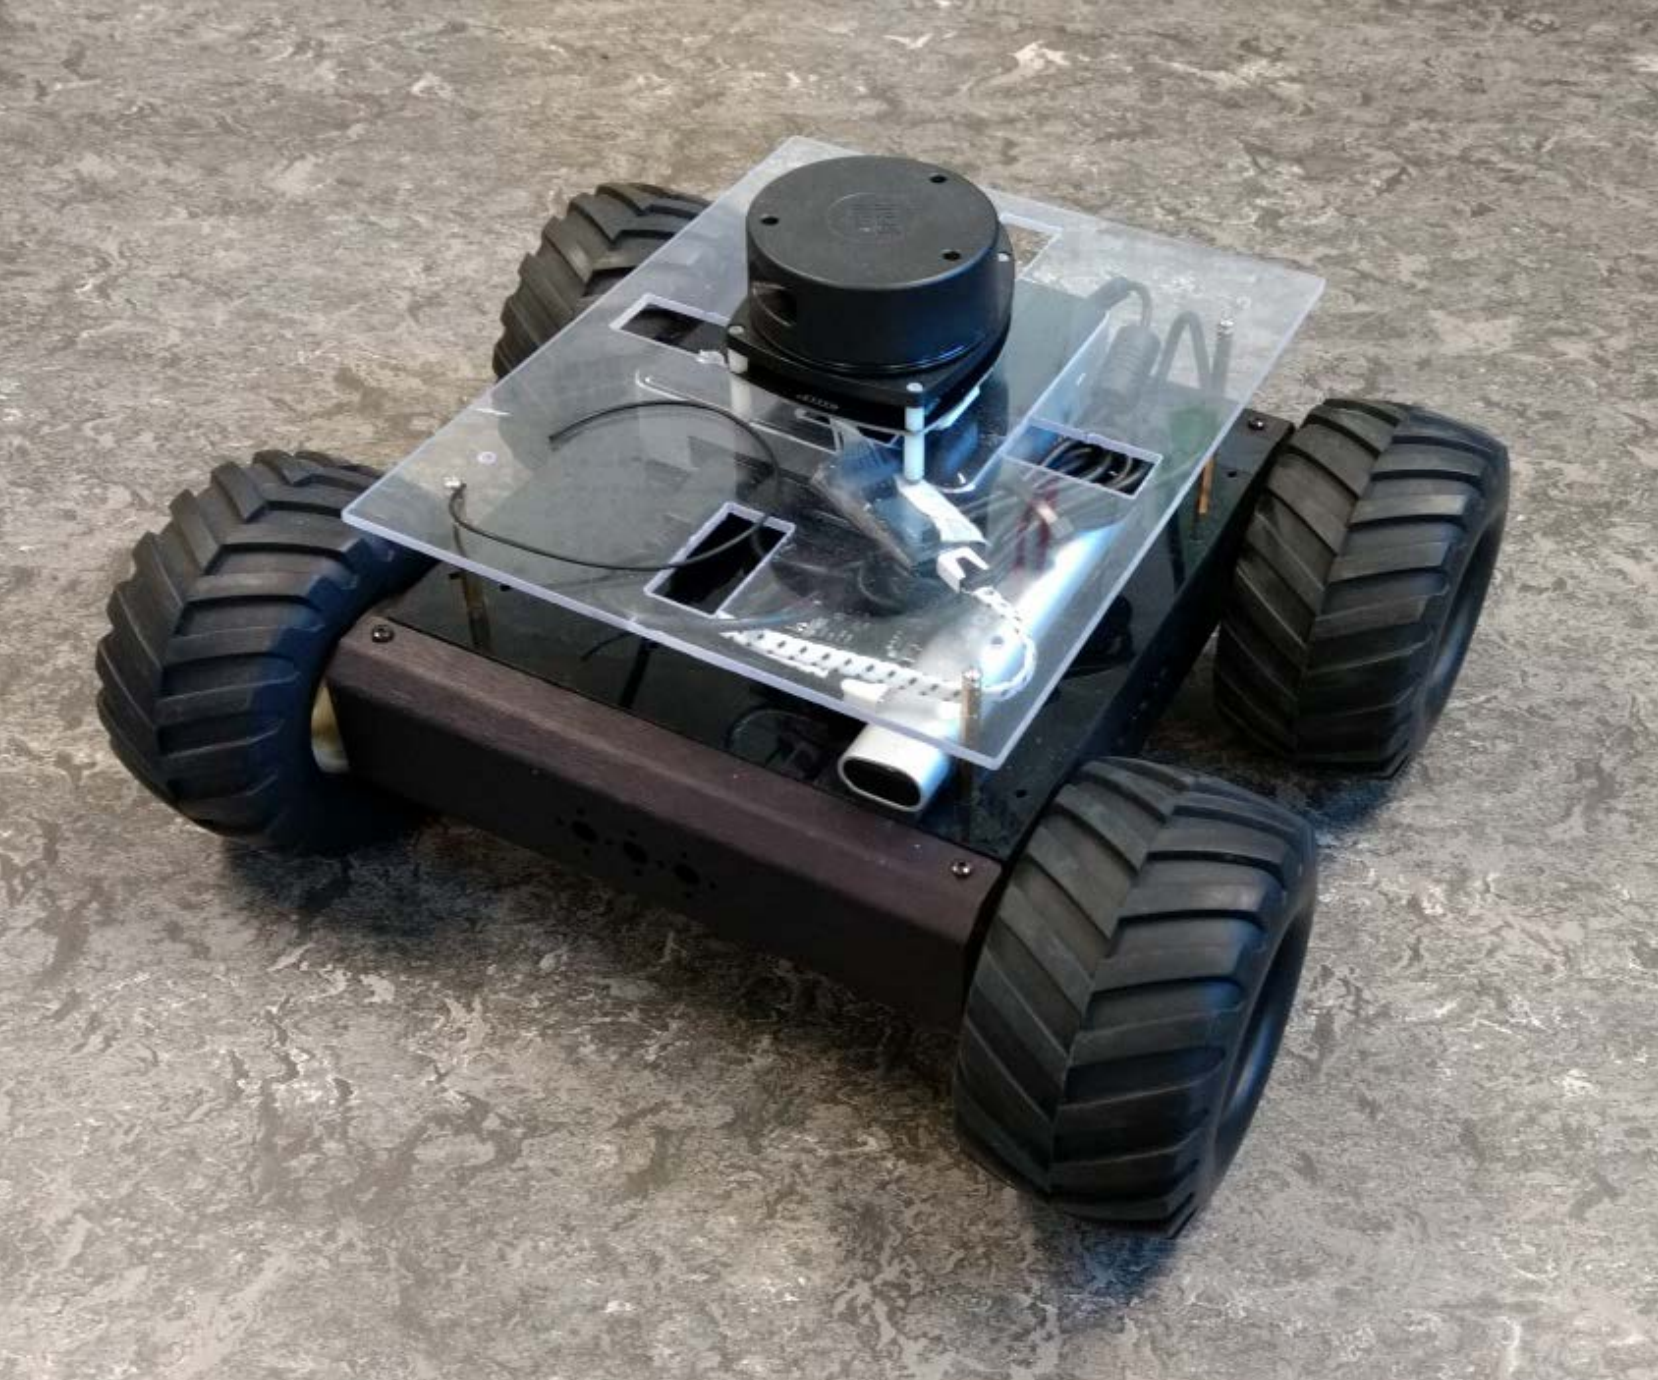
\includegraphics[width=0.5\textwidth]{rover_pic.png}
	\end{figure}
	 
	%----------------------------------------------------------------------------------------
	
	\vfill % Push the date up 1/4 of the remaining page
	
\end{titlepage}

%----------------------------------------------------------------------------------------


\renewcommand{\labelenumi}{\alph{enumi})}


\section{Introduction}
The main goal of this project was to implement motor control, posture regulation and odometric localization in order to get the robot to move do a desired pose. Another important part of the project was to learn about ROS to make it possible to implement ROS nodes for the tasks above.\\
A significant portion of the project time was spent on reverse engineering the robot to better understand the system before we could begin implementing our own solutions.  Most of the work was done in collaboration with the other group, 
as we were working on the same robot while trying to get the system up and running. \\

\section{The System}
Figure 1 shows a block diagram of the system. It consists of posture regulaton, motor controller, kinematic model, and odometry. The following subchapters describes will describe this in more detail.

	\begin{figure}[H]
	\centering
	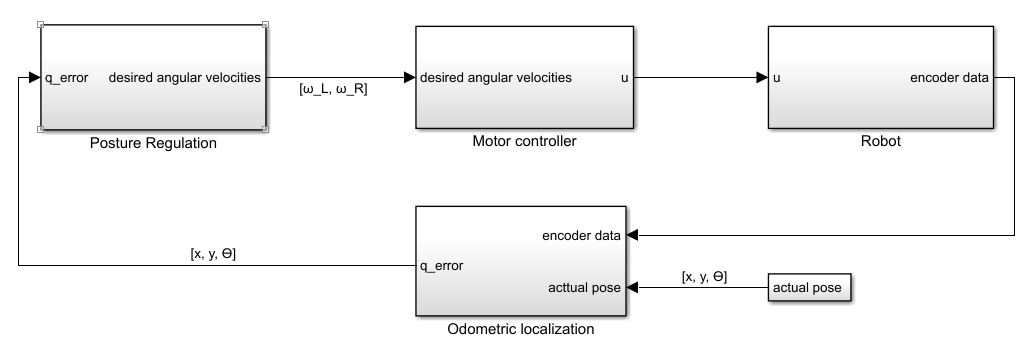
\includegraphics[width=0.9\textwidth]{blokkskjema}
	\caption{Block diagram of the system.}	
 	\label{fig:2}
	\end{figure}

\subsection{Kinematic Model}
We used the kinematic model of a unicycle from page 478 in the book, where $v$ is the driving velocity and $\omega$ is the steering velocity.

\begin{equation}
	\begin{bmatrix}
	\dot{x}\\ 
	\dot{y}\\
	\dot{\theta}\\  
	\end{bmatrix}
	=
	\begin{bmatrix}
	cos\theta\\ 
	sin\theta\\
	0\\  
	\end{bmatrix}v
	+
	\begin{bmatrix}
	0\\ 
	0\\
	1\\  
	\end{bmatrix}\omega
\end{equation}


\subsection{Motor Control}
	We started our project by running and reverse engineering the mobile robot together with the other group.
	As we were not familiar with the system and since there were no README or comments in the code, the challenges for 		reverse engineering the motor controller was: 
	to login, to run robot, understand the controller and deduce the reason behind the constants in the controller.
	The implementation of motor control for each wheel was already avaiable in the robots source. 

\subsection{Odometric Localization}
		
		\begin{equation}
		x_{k+1}=x_k+\frac{v_k}{\omega_k}(sin\theta_{k+1}-sin\theta_k)
		\end{equation}
		\begin{equation}
		y_{k+1}=y_k+\frac{v_k}{\omega_k}(cos\theta_{k+1}-cos\theta_k)
		\end{equation}
		\begin{equation}
		\theta_{k+1}=\theta_k+\omega_kT_s
		\end{equation}
		
\subsection{Posture Regulation}

	
		In general the posture regulation controller takes in the configuration variables, $q = [x, y, \theta]^{T}$, 
		and outputs v and $\omega$.
		It is assumed that the desired variables are $q_{d} = [0, 0, 0]^{T}$ and the error from $q_{d}$ is represented by
		\begin{equation}
			\rho = \sqrt{x^{2} + y^{2}} 
		\end{equation}
		\begin{equation}
			\gamma = Atan2(y, x) - \theta + \pi
		\end{equation}
		\begin{equation}
			\delta = \gamma + \theta
		\end{equation}
		where $\rho = ||\vec{e_{p}}||$ is the distance between current point $(x, y)$ and desired point $(0, 0)$, 
		$\gamma$ is the angle between $\vec{e_{p}}$	and the sagittal axis of the vehicle and $\delta$ is the axis between $\vec{e_{p}}$ and the x-axis.	
		v and $\omega$ are found by:
		\begin{equation}
			v = k_{1}\rho cos(\gamma)
		\end{equation}		
		\begin{equation}
			\omega = k_{2}\gamma + k_{1}\frac{sin(\gamma)cos(\gamma)}{\gamma}(\gamma + k_{3}\delta)
		\end{equation}
		
		In our implementation of the controller we get $\vec{q}$ from the odometric module and output $\omega_{R}$ and $\omega_{L}$ to the motor controller.
		Equations for $\omega_{R}$ and $\omega_{L}$ expressed by error variables $\rho$, $\gamma$ and $\delta$, 
		by setting the following equations (3) and (4) equal to equations (1) and (2) respectively, 
		\begin{equation}
			v = \frac{r(\omega_{R} + \omega_{L})}{2}
		\end{equation}
		\begin{equation}
			\omega = \frac{r(\omega_{R} - \omega_{L})}{d}
		\end{equation}
		and then solve for $\omega_{R}$ and $\omega_{L}$ by the inserting method. This yields:		
		\begin{equation}
			\omega_{R} = \frac{2k_{1}\rho cos(\gamma)}{2r} + \frac{dk{2}\gamma}{2r} + \frac{dsin(\gamma)cos(\gamma)(\gamma + k_{3}\delta)}{2r\gamma}
		\end{equation}
		\begin{equation}
			\omega_{L} = \frac{2k_{1}\rho cos(\gamma)}{2r} - \frac{dk_{2}\gamma}{2r} - \frac{dsin(\gamma)cos(\gamma)(\gamma + k_{3}\delta)}{2r\gamma}
		\end{equation}

\section{Testing and Results}


\end{document}
